\begin{name}
	{\tenchude}
	{\tendethi}
	{\tentruong}
	{\thoigian}
\end{name}
\setcounter{ex}{0}\setcounter{bt}{0}
\TN
\Opensolutionfile{ans}[ans/ansDe4-TN4]
\begin{ex}%[2D1N1-1]
	Cho hàm số $y=\dfrac{x+1}{x-3}$. Trong các mệnh đề sau, mệnh đề nào \textbf{sai}?
	\choice
	{Hàm số nghịch biến trên từng khoảng xác định của nó}
	{\True Hàm số nghịch biến trên tập xác định của nó}
	{Hàm số nghịch biến trên khoảng $(3;+\infty)$}
	{Hàm số nghịch biến trên khoảng $(-\infty; 3)$}
	\loigiai{Hàm số đã cho có tập xác định gồm hai khoảng $(-\infty; 3)$ và $(3;+\infty)$ rời nhau nên khẳng định hàm số nghịch biến trên tập xác định là sai.}
\end{ex}

\begin{ex}%[2D1N1-2]%[CTST- Lớp 12 - Ôn tập cuối học kì 1 - Đề 6]%[Lê Hồng Phi]
	Cho hàm số $y=f(x)$ có bảng biến thiên như sau
	\begin{center}
		
\begin{tikzpicture}
			\tkzTabInit[nocadre=false, lgt=1.2, espcl=2.5, deltacl=0.6]{$x$/0.6,$y'$/0.6,$y$/2}
			{$-\infty$, $-1$, $0$, $1$, $+\infty$}
			\tkzTabLine {,+,0,-,0,+,0,-,}
			\tkzTabVar{-/$-\infty$, +/$2$, -/$1$, +/$2$, -/$-\infty$}
		\end{tikzpicture}
	\end{center}
	Hàm số đã cho đồng biến trên khoảng nào dưới đây?
	\choice
	{$(1;+\infty)$}
	{$(-1;0)$}
	{$(-1;1)$}
	{\True $(0;1)$}
	\loigiai{
		Dựa vào bảng biến thiên thì hàm số đã cho đồng biến trên các khoảng $(-\infty;-1)$ và $(0;1)$.
	}
\end{ex}

\begin{ex}%[2D1V1-5]%[12-EX-TF-TLN-Huyên Nguyễn]
	\immini{
		Hình vẽ bên biểu diễn độ cao của một quả bóng nảy $h$(m) theo thời gian $t$(s). Ta có đồ thị của hàm số $h=-t^2+2t$ trên đoạn $[0;2]$. Nhìn vào hình vẽ, ta suy ra
		\choice
		{Độ cao của quả bóng tăng khi $t\in (0;2)$}
		{ Độ cao của quả bóng tăng khi $t\in (1;2)$}
		{\True Độ cao của quả bóng tăng khi $t\in (0;1)$}
		{Độ cao của quả bóng giảm khi $t\in (0;2)$}
	}
	{\begin{tikzpicture}[>=stealth,line join=round,line cap=round,font=\normalsize,scale=1.5]
			\draw[->] (-0.5,0) -- (2.5,0) node[below] {\scriptsize $t$};
			\draw[->] (0,-0.5) -- (0,1.5) node[left] {\scriptsize $h$};
			\draw (0,0)node[above left]{$O$} ;
			\clip (-0.5,-0.5)rectangle(3,2);
			\draw[smooth,samples=200,domain=0:2] plot (\x,{-(\x)^2+2*(\x)});
			\draw[fill] (0,0) circle(1pt);
			\draw[dashed] (1,0)node[below]{$1$}--(1,1)--(0,1)node[left]{$1$} (2,0)node[below]{$2$};
		\end{tikzpicture}}
	\loigiai{Nhìn đồ thị, ta thấy $h=h(t)$ đồng biến trong $(0;1)$ nên độ cao của quả bóng tăng khi $t\in (0;1)$.}
\end{ex}

\begin{ex}%[2-D1B4-SO-10-2425]%[VN-MT-7, VM012]%[2D1N2-1]
	Giá trị cực tiểu của hàm số $y=f(x)=\dfrac{x^2+x+4}{x+1}$ là
	\choice
	{$y_\text{CT}=-5$}
	{\True $y_\text{CT}=3$}
	{$y_\text{CT}=1$}
	{$y_\text{CT}=-3$}
	\loigiai{
		Tập xác định $\mathscr{D}=\mathbb{R}\setminus\{-1\}$.\\
		Ta có $f'(x)=\dfrac{(2x+1)(x+1)-(x^2+x+4)}{(x+1)^2}=\dfrac{x^2+2x-3}{(x+1)^2}$, $f'(x)=0\Leftrightarrow \hoac{&x=-3\\&x=1.}$\\
		Bảng biến thiên của hàm số:
		\begin{center}
			
\begin{tikzpicture}[scale=1.0, font=\footnotesize, line join=round, line cap=round, >=stealth]
				\tkzTabInit[nocadre=true,espcl=3,lgt=1.5,deltacl=0.5]
				{$x$/0.7,$y'$/0.7,$y$/2.1}
				{$-\infty$,$-3$,$-1$,$1$,$+\infty$}
				\tkzTabLine{,+,0,-,d,-,0,+,}
				\tkzTabVar{-/$-\infty$,+/$-5$,-D+/$-\infty$/$+\infty$,-/$3$,+/$+\infty$}
			\end{tikzpicture}
		\end{center}
		Hàm số đạt cực đại tại $x=-3$ và $y_\text{CĐ}=-5$.\\
		Hàm số đạt cực tiểu tại $x=1$ và $y_\text{CT}=3$.
	}
\end{ex}

\begin{ex}%[2D1N2-2]%[Tổ 24 - Đợt 16 - Chương 1 - - CTST]%[Huỳnh Thanh Chí]
	\immini[thm]{
		Cho hàm số $y=f(x)$ liên tục trên $\mathbb{R}$ và có đồ thị như hình vẽ bên. Hàm số có bao nhiêu điểm cực trị?
		\choice
		{1}
		{2}
		{\True 3}
		{4}
	}{
		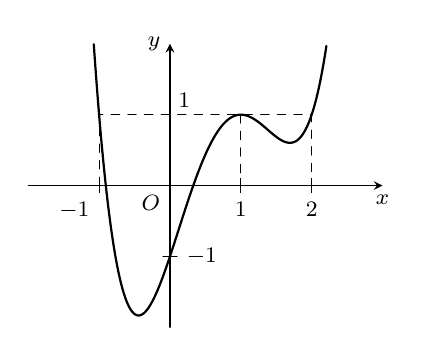
\begin{tikzpicture}[scale=0.9,font=\footnotesize,line join=round,line cap=round,>=stealth]
			\draw[->] (-2,0)--(3,0) node[below] { $x$};
			\draw[->] (0,-2)--(0,2) node[left] { $y$};
			\draw (0,0) node [below left] { $O$};
			\foreach \x in {1,2}\draw (\x,0.1)--(\x,-0.1) node [below] { $\x$};
			\draw (-0.1,-1)--(0.1,-1) node [right] { $-1$}
			(0.2,1.2) node { $1$};
			\draw (-1,0.1)--(-1,-0.1) node [below left] { $-1$}
			;
			\draw[dashed] (-1,0)--(-1,1)--(2,1)--(2,0) (1,1)--(1,0);
			%	\clip (\xmin,\ymin) rectangle (\xmax,\ymax);
			\draw[thick,smooth,samples=200] plot[domain=-1.075:2.21]  (\x,{(\x-2)*(\x-1)^2*(\x+1)+1});
			%	\draw (\xmax,{\f(\xmax)}) node [above right]{$x^4-2x^2+1$};
		\end{tikzpicture}
	}
	\loigiai{Quan sát đồ thị ta thấy hàm số có $3$ điểm cực trị.
	}
\end{ex}

\begin{ex}%[Dự án đề cương thầy Yên]%[Mui Doan]%[2D1H2-1]
	Cho hàm số $y=\dfrac{x^2+3}{x-1}$. Khẳng định nào sau đây là đúng?
	\choice
	{Hàm số đạt cực tiểu tại $x=-1$}
	{\True Hàm số có $2$ cực trị trong đó $y_{CĐ} < y_{CT}$}
	{Hàm số đạt cực đại tại $x=3$}
	{Hàm số có giá trị cực tiểu bằng $-2$}
	\loigiai{
		Tập xác định $\mathscr{D}=\mathbb{R}\setminus\{1\}$.\\
		Ta có $y'=\dfrac{x^2-2x-3}{(x-1)^2}$.\\
		$y'=0\Leftrightarrow\hoac{&x=-1\\&x=3.}$\\
		Bảng biến thiên
		\begin{center}
			\begin{tikzpicture}
				\tkzTabInit[nocadre=false,lgt=1.2,espcl=3,deltacl=0.4]
				{$x$/1, $y'$/0.75, $y$/2}{$-\infty$,$-1$,$1$,$3$,$+\infty$}
				\tkzTabLine{,+,0,-,,-,0,+,}
				\path
				(N13)node[shift={(0,0.2)}](A){$-\infty$}
				(N22)node[shift={(0,-0.4)}](B){$-2$}
				(N33)node[shift={(-0.4,0.2)}](C){$-\infty$}
				(N32)node[shift={(0.4,-0.2)}](D){$+\infty$}
				(N43)node[shift={(0,0.4)}](E){$6$}
				(N52)node[shift={(0,-0.2)}](F){$+\infty$}
				;
				\foreach\X/\Y in{A/B,B/C,D/E,E/F}\draw[-stealth](\X)--(\Y);
				\draw[double](N31) --(N33);
			\end{tikzpicture}
		\end{center}
		Vậy hàm số có $2$ cực trị trong đó $y_{CĐ} < y_{CT}$.
	}
\end{ex}

\begin{ex}%[2D1H3-1]
	Tìm giá trị nhỏ nhất của hàm số $y = 2\cos^2 x - 3\cos x + 1$ trên tập xác định $\mathbb{R}$.
	\choice
	{$\dfrac{1}{3}$}
	{$\dfrac{1}{4}$}
	{\True $-\dfrac{1}{8}$}
	{Không tồn tại}
	\loigiai{
		Đặt $t = \cos x$, $t \in [-1;1]$. Khi đó hàm số trở thành $f(t) = 2t^2 - 3t + 1$.\\
		Ta có $f'(t) = 4t - 3 = 0 \Leftrightarrow t = \dfrac{3}{4} \in [-1;1]$.\\
		Tính được các giá trị $f(-1) = 6$, $f\left(\dfrac{3}{4}\right) = -\dfrac{1}{8}$, $f(1) = 0$.\\
		Từ đây, giá trị nhỏ nhất của hàm số đã cho là $-\dfrac{1}{8}$.
	}
\end{ex}

\begin{ex}%[2D1N4-1]%[EX-TF-TLN-2024-Huyên Nguyễn]
	Mặt cầu $S$ tâm $I(a;b;c)$, bán kính $R>0$ có phương trình là
	\choice
	{$(x+a)^2+(y+b)^2+(z+c)^2=R^2$}
	{\True $(x-a)^2+(y-b)^2+(z-c)^2=R^2$}
	{$(x-a)+(y-b)+(z-c)=R$}
	{$|x+a|+|y+b|+|z+c|=R^2$}
	\loigiai
	{Mặt cầu $S$ tâm $I(a;b;c)$ và bán kính $R$ có phương trình là  $(x-a)^2+(y-b)^2+(z-c)^2=R^2$.}
\end{ex}

\begin{ex}%[2-D1B5-SO-15-2425]%[VN-MT-7, Đoàn Thị Lý]%[2D1H4-1]
	Đồ thị hàm số $y=\dfrac{x^2-3 x-4}{x^2-16}$ có bao nhiêu đường tiệm cận đứng?
	\choice
	{\True $1$}
	{$0$}
	{$2$}
	{$3$}
	\loigiai{
		Tập xác định $\mathscr{D}=\mathbb{R} \setminus\big\{- 4;4\big\}$. Ta có
		\begin{itemize}
			\item $\lim\limits _{x \to (-4)^-} y=\lim\limits _{x \to (-4)^-} \dfrac{x^2-3 x-4}{x^2-16}=\lim\limits _{x \to (-4)^-} \dfrac{(x+1)(x-4)}{(x+4)(x-4)}=\lim\limits _{x \to (-4)^-} \dfrac{x+1}{x+4}=+\infty$, suy ra $x=-4$ là tiệm cận đứng của đồ thị hàm số.
			\item $\lim\limits_{x \to 4} y=\lim\limits _{x \to 4} \dfrac{x^2-3 x-4}{x^2-16}=\lim\limits _{x \to 4} \dfrac{(x+1)(x-4)}{(x+4)(x-4)}=\lim\limits _{x \to 4} \dfrac{x+1}{x+4}=\dfrac{5}{8}$, suy ra $x=4$ không là tiệm cận đứng của đồ thị hàm số.
		\end{itemize}
		Vậy đồ thị hàm số có $1$ đường tiệm cận đứng.
	}
\end{ex}

\begin{ex}%[2D1V4-1]
	Cho $y=f(x)$ là hàm số bậc ba, liên tục trên $\mathbb{R}$. Đồ thị hàm số $g(x)=\dfrac{1}{f(x^3+3x)-1}$ có nhiều nhất bao nhiêu đường tiệm cận.
	\choice
	{\True $4$} {$2$} {$5$} {$3$}
	\loigiai{
		Đặt $t=x^3+3x \Rightarrow t'=3x^2+3>0,\forall x \in\mathbb{R}$.\\
		Ta có bảng biến thiên:
		\begin{center}
			
\begin{tikzpicture}[scale=1, font=\footnotesize, line join=round, line cap=round, >=stealth]
				\tkzTabInit[nocadre=false,lgt=2,espcl=2,deltacl=0.6]
				{$x$ /0.6,$t'$ /0.6,$t$ /2}
				{$-\infty$, $+\infty$}
				\tkzTabLine{,+,}
				\tkzTabVar{-/ $-\infty$ , +/$+\infty$}
			\end{tikzpicture}
		\end{center}
		Xét $f(x^3+3x)-1=0$. Vì $y=f(x)$ là hàm số bậc ba nên phương trình $f(t)=1$ có nhiều nhất $3$ nghiệm $t$.\\
		Từ bảng biến thiên ta suy ra với mỗi giá trị $t$ có đúng một giá trị $x$.\\
		Khi đó phương trình $f(x^3+3x)=1$ có nhiều nhất $3$ tiệm cận đứng.\\
		Do đó đồ thị hàm số $y=g(x)$ có nhiều nhất $3$ tiệm cận đứng.\\
		Xét $\underset{x \to\pm\infty}{\lim}g(x) = \underset{x \to\pm\infty}{\lim}\dfrac{1}{f(x^3+3x)-1}= \underset{x \to\pm\infty}{\lim}\dfrac{1}{f(t)-1}=0$ $(\text{vì}\underset{x \to\pm\infty}{\lim}f(t)=\pm\infty)$.\\
		Suy ra đồ thị hàm số $y=g(x)$ có $1$ tiệm cận ngang là $y=0$.\\
		vậy đồ thị hàm số $y=g(x)$ có nhiều nhất $4$ đường tiệm cận.
	}
\end{ex}

\begin{ex}%[Dự án Giảng 12 Nhóm Toán & LaTex, Lê Minh Thiện Anh]%[2D1N5-1]
	\immini{Bảng biến thiên ở hình bên là của một trong bốn hàm số sau đây. Hỏi đó là hàm số nào?
		\choice
		{$y=-x^3-2x^2+5$}
		{\True $y=x^3-3x^2+5$}
		{$y=-x^3-3x+5$}
		{$y=x^3+3x^2+5$}}{
		
\begin{tikzpicture}
			\tkzTabInit[nocadre=false, lgt=1.2,espcl=2.5]{$x$ /0.6,$y'$ /0.6,$y$ /2}{$-\infty$,$0$,$2$,$+\infty$}
			\tkzTabLine{,+,$0$,-,$0$,+,}
			\tkzTabVar{-/ $-\infty$/, +/$5$ , -/$1$  , +/$+\infty$/}
		\end{tikzpicture}}
	\loigiai{
		Quan sát BBT, ta thấy $\lim\limits_{x\rightarrow +\infty}y=+\infty$, suy ra hệ số $a>0$ nên loại phương án $y=-x^3-2x^2+5$ và $y=-x^3-3x+5$.
		Mặt khác, đồ thị đi qua điểm $(2;1)$ nên chọn hàm $y=x^3-3x^2+5$.
	}
\end{ex}

\begin{ex}%[Dự Án Giảng 12 4 in 1, Lê Văn Toàn]%[2D1N5-7]
	Cho đồ thị hàm số $y=\dfrac{2x-1}{x+2}$ có đồ thị $(C)$. Tọa độ điểm $I$ là tâm đối xứng của đồ thị hàm số là
	\choice
	{\True $I(-2;2)$}
	{$I\left(-2;-\dfrac{1}{2}\right)$}
	{$I(2;2)$}
	{$I\left(2;\dfrac{1}{2}\right)$}
	\loigiai{
		Đồ thị hàm số có tiệm cận đứng $x=-2$, tiệm cận ngang $y=2$.\\
		Tâm đối xứng của đồ thị hàm số là điểm $I$ có tọa độ $(-2;2)$.
	}
\end{ex}

\begin{ex}%[2D1H5-1]
	Hàm số nào dưới đây có bảng biến thiên như sau?
	\begin{center}
		
\begin{tikzpicture}
			\tkzTabInit[lgt=1.2,espcl=2]
			{$x$ /0.8, $y'$ /0.8, $y$ /1.8}
			{$-\infty$,$-2$,$1$,$+\infty$}
			\tkzTabLine{ ,+,z,-,z,+ }
			\tkzTabVar{-/$-\infty$,+/$20$,-/$-7$,+/$+\infty$}
		\end{tikzpicture}
	\end{center}
	\choice
	{$y=-2x^3-3x^2+12x$}
	{\True $y=2x^3+3x^2-12x$}
	{$y=-2x^4-3x^2+12x$}
	{$y=2x^3-3x^2+12x$}
	\loigiai{
		Dựa vào bảng biến thiên, hàm số cần tìm có dạng $y=ax^3+bx^2+cx+d$ với hệ số $a>0$. Do đó đáp án đúng chỉ có thể là $y=2x^3+3x^2-12x$ hoặc $y=2x^3-3x^2+12$.\\
		Xét hàm số $y=2x^3+3x^2-12x$ có $y'=6x^2+6x-12$.\\
		$y'=0 \Leftrightarrow 6x^2+6x-12=0 \Leftrightarrow \hoac{&x=1\\&x=-2.}$\\
		Bảng biến thiên
		\begin{center}
			
\begin{tikzpicture}
				\tkzTabInit[lgt=1.2,espcl=2]
				{$x$ /0.8, $y'$ /0.8, $y$ /1.8}
				{$-\infty$,$-2$,$1$,$+\infty$}
				\tkzTabLine{ ,+,z,-,z,+ }
				\tkzTabVar{-/$-\infty$,+/$20$,-/$-7$,+/$+\infty$}
			\end{tikzpicture}
		\end{center}
	}
\end{ex}

\begin{ex}%[Dự án 2025_K12_TL TV]%[Phạm Thị Thanh Thuỷ]%[2D1V5-8]
	Một vật chuyển động có đồ thị của hàm quãng đường $s(t)$, hàm vật tốc $v(t)$ và hàm gia tốc $a(t)$ theo thời gian $t$ được mô tả ở hình dưới đây. Khẳng định nào dưới đây \textbf{đúng}?
	\begin{center}
		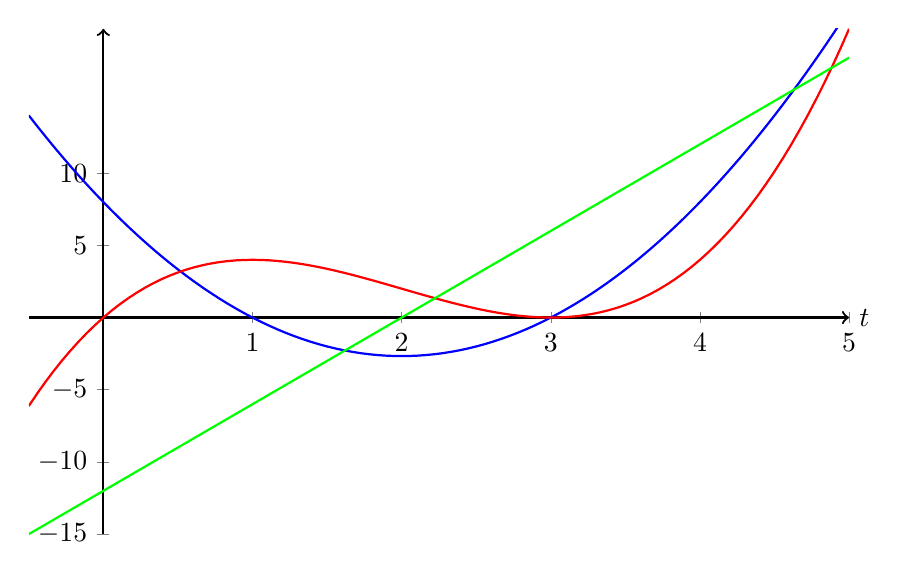
\begin{tikzpicture}
			\begin{axis}[
					width=12cm,
					height=8cm,
					xlabel={$t$},
					ylabel={},
					axis lines=middle,
					xtick={0, 1, 2, 3,4,5},
					ytick={-15,-10,-5, 0, 5,10},
					ymin=-15, ymax=20,
					xmin=-0.5, xmax=5,
					domain=-0.5:5,
					samples=100,
					axis line style={->},
					every axis x label/.style={at={(ticklabel* cs:1)},anchor=west},
					every axis y label/.style={at={(ticklabel* cs:1)},anchor=south},
					thick,
					legend pos=outer north east
				]

				% Plotting the three functions
				\addplot[blue, thick] {8/3* x^2 - 32/3 *x + 8};
				\addplot[red, thick] {x^3 - 6*x^2 + 9*x};
				\addplot[green, thick] {6*x - 12};
			\end{axis}
		\end{tikzpicture}
	\end{center}
	\choice
	{\True $s(4)<v(4)<a(4)$}
	{$a(4)<v(4)<s(4)$}
	{$s(4)<a(4)<v(4)$}
	{$v(4)<a(4)<s(4)$}
	\loigiai{
		\begin{enumerate}
			\item Xác định các hàm trên đồ thị\\
			      - Đồ thị của gia tốc $a(t)$ dao động nhanh nhất và có biên độ lớn nhất.\\
			      - Đồ thị của vận tốc $v(t)$ dao động nhanh vừa phải.\\
			      - Đồ thị của vị trí $s(t)$ dao động chậm nhất.
			\item Phân tích đồ thị trong hình ảnh\\
			      - Đường cong màu xanh lá dao động nhanh nhất và có biên độ lớn nhất, điều này phù hợp với hàm gia tốc $a(t)$.\\
			      - Đường cong màu xanh dương dao động nhanh vừa phải, điều này phù hợp với hàm vận tốc $v(t)$.\\
			      - Đường cong màu đỏ dao động chậm nhất, điều này phù hợp với hàm quãng đường $s(t)$.
			\item Đánh giá giá trị các hàm tại $t=4$ ta được $s(4)<v(4)<a(4)$.
		\end{enumerate}
	}
\end{ex}

\begin{ex}%[Dự án Đề Cương 12-Thầy Vỹ,Mui Doan]%[2D1H3-6]
	Có một tấm nhôm hình vuông cạnh $12cm.$ Người ta cắt ở bốn góc của tấm nhôm đó bốn hình vuông bằng nhau, mỗi hình vuông có cạnh bằng $x$ (cm) rồi gấp tấm nhôm lại như hình vẽ dưới đây để được một cái hộp không nắp. Tìm $x$ để hình hộp nhận được có thể tích lớn nhất.
	\choice
	{$x=6$}
	{$x=3$}
	{\True $x=2$}
	{$x=4$}
	\loigiai{
		Độ dài cạnh đáy của cái hộp là $12-2x$.\\
		Diện tích đáy của cái hộp là $(12-2x)^2$.\\
		Thể tích cái hộp là $V(x)=(12-2x)^2\cdot x=4x^3-48x^2+144x$ với $x\in (0;6)$.\\
		Ta có $V'(x)=12x^3-96x^2+144x$.\\
		Cho $V'(x)=0\Leftrightarrow \hoac{&x=0~\text{(loại)}\\&x=2~\text{(nhận)}\\&x=6~\text{(loại)}.}$\\
		Bảng biến thiên
		\begin{center}
			\begin{tikzpicture}[font=\normalsize,t style/.style={style=solid}]
				\tkzTabInit[nocadre=true,lgt=1.2,espcl=3,deltacl=0.5]
				{$x$ /0.75, $V'(x)$/0.75, $V(x)$/2.5}
				{$0$,$2$,$6$}
				\tkzTabLine{  , +,0 , -,  }
				\path ($(N12)!0.9!(N13)$) node (A1){$0$}
				($(N22)!0.2!(N23)$) node (A2){$128$}
				($(N32)!0.9!(N33)$) node (A3){$0$};
				\foreach \x/\y in {A1/A2,A2/A3}{
						\draw[-stealth] (\x)--(\y);
					}
			\end{tikzpicture}
		\end{center}
		Ta được $V_{\max}=128$ khi $x=2$.
	}
\end{ex}

\begin{ex} %[2D1H2-7]
	Giả sử chi phí tiền xăng C (đồng) phụ thuộc tốc độ trung bình  $v\left( {{\rm{\;km}}/{\rm{h}}} \right)$ theo công thức
	\[C(v) = \dfrac{16000}{v} + \dfrac{5}{2}v \quad (0 < v \le 120)\]
	Tính tốc độ trung bình để chi phí tiền xăng đạt cực tiểu.
	\choice
	{$60$ km/h}
	{$70$ km/h}
	{$50$ km/h}
	{\True $80$ km/h}
	\loigiai{
		Tập xác định: $D=(0; 120]$.\\
		Đạo hàm $C'(v)=-\dfrac{16000}{v^2}+\dfrac{5}{2}=\dfrac{5(v-80)(v+80)}{2v^2}$; $C'(v)=0\Leftrightarrow v=-80$ (loại) hoặc $v=80$.\\
		Bảng biến thiên
		\begin{center}
			
\begin{tikzpicture}[>=stealth]
				\tkzTabInit[nocadre=false,lgt=1.5,espcl=2,deltacl=0.5]{$v$/.7 ,$C'(v)$/.7,$C(v)$/2}
				{$0$ , $80$ , $120$}
				\tkzTabLine{ d, - , $0$ , + , }
				\tkzTabVar{+D+/$ $/$+\infty$ , -/$400$ , +/$\dfrac{1300}{3}$}
			\end{tikzpicture}
		\end{center}
		Quan sát bảng biến thiên, ta nhận thấy hàm số đạt cực tiểu khi $v=80$.\\
		Như vậy, để chi phí tiền xăng đạt cực tiểu, tài xế nên chạy xe với tốc độ trung bình là $80$ km/h.
	}
\end{ex}

\begin{ex}%[2-H2B4-SO-11-2425]%[VN-MT-7, Đào Trung Kiên]%[2H2N1-1]
	Cho hình lập phương $ABCD.A'B'C'D'$ có cạnh là $a$. Vectơ nào bằng vectơ $\overrightarrow{D'C'}$?
	\choice{$\overrightarrow{DD'}$}
	{$\overrightarrow{AD}$}
	{\True $\overrightarrow{AB}$}
	{$\overrightarrow{CD}$}
	\loigiai{
		\begin{center}
			\begin{tikzpicture}[font=\footnotesize, line join=round, line cap=round, >=stealth, scale=1]
				\def\a{3.5}
				\path (0:0) coordinate (A)
				++(0:\a) coordinate (B)
				++(-130:\a/2) coordinate (C)
				($(A)+(C)-(B)$) coordinate (D)
				($(A)+(-90:\a)$) coordinate (A')
				($(B)+(-90:\a)$) coordinate (B')
				($(C)+(-90:\a)$) coordinate (C')
				($(D)+(-90:\a)$) coordinate (D');
				\draw[dashed] (B)--(A) (A)--(A')--(B') (A')--(D');
				\draw[->] (A)--(B);
				\draw[->] (D')--(C');
				\draw (C)--(C')--(B') (A)--(D)--(D') (A)--(B)--(B') (B)--(C)--(D) ;
				\foreach \x/\g in {A/180,D/180,C/0,B/0,A'/180,D'/180,C'/0,B'/0}
				\fill (\x) circle (1pt)
				($(\g:4mm)+(\x)$) node {$\x$};
			\end{tikzpicture}
		\end{center}
		Vì hai vectơ $\overrightarrow{AB}$ và $\overrightarrow{D'C'}$ có cùng hướng và cùng độ dài nên $\overrightarrow{AB}=\overrightarrow{D'C'}$.
	}
\end{ex}

\begin{ex}%[2H2N1-2]
	Cho hình hộp $ ABCD.A'B'C'D' $. Lấy $ M $ là trung điểm của đoạn thẳng $ CC' $. Véc-tơ $ \vec{AM} $ bằng
	\choice
	{$ \vec{AB}+\vec{AD}+\vec{AA'} $}
	{\True $ \vec{AB}+\vec{AD}+\dfrac{1}{2}\vec{AA'} $}
	{$ \vec{AB}+\dfrac{1}{2}\vec{AD}+\dfrac{1}{2}\vec{AA'} $}
	{$ \dfrac{1}{2}\vec{AB}+\vec{AD} +\vec{AA'} $}
	\loigiai{
		\begin{center}
			\begin{tikzpicture}[scale=1, font=\footnotesize, line join=round, line cap=round, >=stealth]
				\def\bc{4} % cạnh BC
				\def\ba{2} % cạnh BA
				\def\h{4} % đường cao
				\def\gocB{35} % góc B của đáy
				\coordinate[label=below left:$B$] (B) at (0,0);
				\coordinate[label=above left:$A$] (A) at (\gocB:\ba);
				\coordinate[label=below:$C$] (C) at (\bc,0);
				\coordinate[label=right:$D$] (D) at ($(C)-(B)+(A)$);
				\coordinate[label=above left:$A'$] (A') at ($(A)+(90:\h)$);
				\coordinate[label=left:$B'$] (B') at ($(B)-(A)+(A')$);
				\coordinate[label=below right:$C'$] (C') at ($(C)-(A)+(A')$);
				\coordinate[label=right:$D'$] (D') at ($(D)-(A)+(A')$);
				\coordinate[label=right:$M$] (M) at ($(C)!0.5!(C')$);
				\draw (B')--(B)--(C)--(D)--(D')--(A')--(B')--(C')--(D') (C)--(C');
				\draw[dashed] (A')--(A)--(D) (M)--(A)--(B);
				\foreach \diem in {A,B,C,D,A',B',C',D',M}	\fill (\diem)circle(1.5pt);
			\end{tikzpicture}
		\end{center}
		Ta có $ \vec{AM}=\vec{AC}+\vec{CM} = \vec{AB}+\vec{AD}+\vec{CM}= \vec{AB}+\vec{AD}+\dfrac{1}{2}\vec{AA'}$.
	}
\end{ex}

\begin{ex}%[2H2H1-3]
	\immini{Cho hình lập phương $ABCD.A'B'C'D'$ cạnh bằng $2a$. Tính góc giữa hai véc-tơ $\overrightarrow{AC'}$ và $\overrightarrow{BD}$.
		\choice
		{$120^\circ$}
		{$45^\circ$}
		{\True $90^\circ$}
		{$60^\circ$}
	}{\begin{tikzpicture}[line join=round,line cap=round,>=stealth,scale=0.5,font=\footnotesize]
			\foreach \x/\y/\n in {0/0/A,-1.5/-2/B,5/0/D} \coordinate (\n) at (\x,\y);
			\coordinate (C) at ($(B)+(D)-(A)$);
			\foreach \x/\y in {A/A',B/B',C/C',D/D'} \coordinate (\y) at ($(\x)+(0,3.5)$);
			\draw (A')--(B')--(C')--(D')--(A') (B')--(B)--(C)--(D)--(D') (C)--(C');
			\draw[dashed] (A')--(A)--(D) (A)--(B) (A)--(C) (B)--(D) (A)--(C');
			\foreach \t/\g in {A/-90,B/-150,C/-30,D/30,A'/90,B'/150,C'/-20,D'/60}{
					\fill (\t) circle(1.5pt) node[shift={(\g:7pt)}]{$ \t $};
				}
		\end{tikzpicture}}
	\loigiai{
		Ta có $\overrightarrow{AC'}\cdot\overrightarrow{BD}=\left(\overrightarrow{AC}+\overrightarrow{CC'}\right)\cdot\overrightarrow{BD}=\overrightarrow{AC}\cdot\overrightarrow{BD}+\overrightarrow{CC'}\cdot\overrightarrow{BD}=0+0=0$.\\
		Suy ra $\overrightarrow{AC'}\perp\overrightarrow{BD}$.
	}
\end{ex}

\begin{ex}%[2-H2B1-SO-3-2425]%[VN-MT-7,VM017]%[2H2H1-2]
	\immini{Cho lập phương $ABCD.A'B'C'D'$ có độ dài mỗi cạnh bằng $1$. Tính độ dài của vectơ $\overrightarrow{AC}+\overrightarrow{C'D'}$.
		\choice
		{$\sqrt{3}$}
		{$\sqrt{2}$}
		{\True $1$}
		{$2\sqrt{2}$}}
	{
		\begin{tikzpicture}[scale=1, font=\footnotesize, line join=round, line cap=round, >=stealth]
			\def\a{3}
			\def\b{2}
			\def\h{3}
			\path (0:0) coordinate (A)
			++(0:\a) coordinate (D)
			++(-130:\b) coordinate (C)
			($(A)+(C)-(D)$) coordinate (B)
			($(A)+(90:\h)$) coordinate (A')
			($(B)+(90:\h)$) coordinate (B')
			($(C)+(90:\h)$) coordinate (C')
			($(D)+(90:\h)$) coordinate (D');
			\draw[dashed] (B)--(A)--(D) (A)--(A') (A)--(C);
			\draw (C)--(C') (D)--(D') (B)--(B') (C)--(C')--(A')
			(B)--(C)--(D)
			(A')--(B')--(C')--(D')--cycle;
			\foreach \x/\g in {A/180,B/180,C/0,D/0,A'/180,B'/180,C'/0,D'/0}
			\fill (\x) circle (1pt)
			($(\g:4mm)+(\x)$) node {$\x$};
		\end{tikzpicture}
	}
	\loigiai{
		Ta có: $A'C'CA$ là hình chữ nhật nên $\overrightarrow{A'C'}=\overrightarrow{AC}$.\\
		Khi đó, $\overrightarrow{AC}+\overrightarrow{C'D'}=\overrightarrow{A'C'}+\overrightarrow{C'D'}=\overrightarrow{A'D'}$.\\
		Vậy $\left|\overrightarrow{AC}+\overrightarrow{C'D'}\right|=\left|\overrightarrow{A'D'}\right|=A'D'=1$.
	}
\end{ex}

\begin{ex}%[2H2H1-3]
	Trong không gian $Oxyz$, cho hai điểm $A(1;-2;1)$ và $B(2;1;1)$. Đoạn thẳng $AB$ có độ dài bằng
	\choice
	{\True $\sqrt{10}$}
	{$10$}
	{$\sqrt{2}$}
	{$2$}
	\loigiai{
		Ta có $AB=\sqrt{(2-1)^{2}+(1--2)^{2}+(1-1)^{2}}=\sqrt{10}$.
	}
\end{ex}

\begin{ex}%[2-H2B1-SO-3-2425]%[VN-MT-7,VM017]%[2H2H1-1]
	\immini[thm]{Cho hình hộp chữ nhật $ABCD.A'B'C'D'$. Trong các vectơ dưới đây, vectơ nào cùng phương với vectơ $\overrightarrow{AB}$?
		\choice
		{Vectơ $\overrightarrow{AD}$}
		{Vectơ $\overrightarrow{CC'}$}
		{Vectơ $\overrightarrow{BD}$}
		{\True Vecto $\overrightarrow{CD}$}}
	{
		\begin{tikzpicture}[scale=0.7, font=\footnotesize, line join=round, line cap=round, >=stealth]
			\def\a{3}
			\def\b{2}
			\def\h{3.5}
			\path (0:0) coordinate (A)
			++(0:\a) coordinate (D)
			++(-130:\b) coordinate (C)
			($(A)+(C)-(D)$) coordinate (B)
			($(A)+(90:\h)$) coordinate (A')
			($(B)+(90:\h)$) coordinate (B')
			($(C)+(90:\h)$) coordinate (C')
			($(D)+(90:\h)$) coordinate (D');
			\draw[dashed] (B)--(A)--(D) (A)--(A');
			\draw (C)--(C') (D)--(D') (B)--(B') (C)--(C')
			(B)--(C)--(D)
			(A')--(B')--(C')--(D')--cycle;
			\foreach \x/\g in {A/180,B/180,C/0,D/0,A'/180,B'/180,C'/0,D'/0}
			\fill (\x) circle (1pt)
			($(\g:4mm)+(\x)$) node {$\x$};
		\end{tikzpicture}
	}
	\loigiai{
		Giá của vectơ $\overrightarrow{AB}$ là đường thẳng $AB$.\\
		Giá của vectơ $\overrightarrow{CD}$ là đường thẳng $CD$.\\
		Mà $AB \parallel CD$.\\
		Do đó vectơ $\overrightarrow{AB}$ cùng phương với vectơ $\overrightarrow{CD}$.
	}
\end{ex}

\begin{ex}%[2H2V1-3]
	Trong không gian $Oxyz$, cho hai véc-tơ $\overrightarrow{u}$ và $\overrightarrow{v}$ tạo với nhau một góc $120^{\circ}$ và $\left|{\overrightarrow{u}}\right|=2$, $\left|{\overrightarrow{v}}\right|=5$. Tính $\left|{\overrightarrow{u} + \overrightarrow{v}}\right|$?

	\choice
	{\True $\sqrt{19}$}
	{$-5$}
	{$7$}
	{$\sqrt{39}$}

	\loigiai{
		\begin{equation}
			\begin{split}
				{\left( {\left| {\overrightarrow u  + \overrightarrow v } \right|} \right)^2} & = {\left( {\overrightarrow u  + \overrightarrow v } \right)^2} = {\overrightarrow u ^2} + 2\overrightarrow u \overrightarrow v  + {\overrightarrow v ^2}                                                                 \\
				                                                                              & = {\left| {\overrightarrow u } \right|^2} + 2\left| {\overrightarrow u } \right|\left| {\overrightarrow v } \right|\cos \left( {\overrightarrow u ;\overrightarrow v } \right) + {\left| {\overrightarrow v } \right|^2} \\ &= {2^2} + 2 \times 2 \times 5 \times \left( { - \dfrac{1}{2}} \right) + {5^2} = 19
			\end{split}
		\end{equation}
	}

\end{ex}

\begin{ex}%[2-H2B4-SO-13-2425 (Nguồn Đề 13 - )]%[VN-MT-7, Lê Văn Hiếu]%[2H2N2-2]
	Trong không gian $Oxyz$, cho hai điểm $A(-3;2;-1)$, $B(-1;0;5)$. Tọa độ trung điểm $I$ của đoạn thẳng $AB$ là
	\choice
	{$I(-1;1;2)$}
	{$I(2;1;-2)$}
	{$I(-2;-1;2)$}
	{\True $I(-2;1;2)$}
	\loigiai{Tọa độ trung điểm $I$ của đoạn thẳng $AB$ là $I(-2;1;2)$.
	}\end{ex}

\begin{ex}%[Đề chuẩn hóa- Kiểm tra chương 2]%[Nguyễn Thành Nhân]%[2H2N2-1]
	Trong không gian $Oxyz$, cho hai điểm $A(-1;2;3)$ và $B(3;0;-2)$. Tìm tọa độ của véc-tơ $\overrightarrow{AB}$.
	\choice
	{$\overrightarrow{AB}=\left(-4;2;5\right)$}
	{$\overrightarrow{AB}=\left(1;1;\dfrac{1}{2}\right)$}
	{$\overrightarrow{AB}=\left(2;2;1\right)$}
	{\True $\overrightarrow{AB}=\left(4;-2;-5\right)$}
	\loigiai{
		Ta có $\overrightarrow{AB}=\left(4;-2;-5\right)$.
	}
\end{ex}

\begin{ex}%[Trần Quang Trường-Hình học 12-Chương 2]%[2H2H2-4]
	Trong không gian với hệ trục tọa độ $Oxyz$, cho véc-tơ $\overrightarrow{u}=(1;1;-2)$, $\overrightarrow{v}=(1;0;m)$. Tìm $m$ để góc giữa hai $\overrightarrow{u}$, $\overrightarrow{v}$ bằng $45^{\circ}$.
	\choice
	{$m=2$}
	{\True $m=2-\sqrt{6}$}
	{$m=2+\sqrt{6}$}
	{$m=2 \pm \sqrt{6}$}
	\loigiai{
		\allowdisplaybreaks
		\begin{eqnarray*}
			\text{Ta có } \cos(\overrightarrow{u},\overrightarrow{v})&=& \dfrac{\overrightarrow{u}\cdot\overrightarrow{v}}{\left|\overrightarrow{u}\right|\cdot\left|\overrightarrow{v}\right|}=\dfrac{1-2m}{\sqrt{1^2+1^2+(-2)^2}\cdot\sqrt{1^2+m^2}}=\dfrac{1-2m}{\sqrt{6}\cdot\sqrt{1+m^2}}=\dfrac{\sqrt 2}{2}\\
			\Leftrightarrow 1-2m&=&\sqrt{3}\cdot\sqrt{1+m^2}
			\Leftrightarrow 4m^2-4m+1=3+3m^2\Leftrightarrow \hoac{&m=2-\sqrt{6}\\&m=2+\sqrt{6}} \quad(m<\dfrac{1}{2})
		\end{eqnarray*}
		Đối chiếu điều kiện ta có $m=2-\sqrt{6}$.
	}
\end{ex}

\begin{ex}%[2H2H2-1]
	Trong không gian với hệ tọa độ $Oxyz$, cho các véc-tơ $\vec{a}=\left( 2;-2;-4 \right)$ và $\vec{b}=\left( 1;-1;1 \right)$. Mệnh đề nào dưới đây \textbf{sai}?
	\choice
	{$\vec{a}+\vec{b}=\left( 3;-3;-3 \right)$}
	{$\vec{a} \perp \vec{b}$}
	{$|\vec{b}|=\sqrt{3}$}
	{\True $\vec{a}$ và $\vec{b}$ cùng phương}
	\loigiai{Vì $\dfrac{2}{1}=\dfrac{-2}{-1} \neq \dfrac{-4}{1}$ nên $\vec{a}$ và $\vec{b}$ không cùng phương.}
\end{ex}

\begin{ex}%[Đề chuẩn hóa- Kiểm tra chương 2]%[Nguyễn Thành Nhân]%[2H2H2-4]
	Trong không không gian $Oxyz$, cho hai véctơ $\overrightarrow{u}=(2;3 ;-1)$ và $\overrightarrow{v}=(5;-4;m)$. Tìm $m$ để $\overrightarrow{u}\perp \overrightarrow{v}$.
	\choice
	{\True $m=-2$}
	{$m=2$}
	{$m=0$}
	{$m=4$}
	\loigiai{
		Ta có $\overrightarrow{u} \perp \overrightarrow{v}\Leftrightarrow 2\cdot5-3\cdot4-m=0 \Leftrightarrow m=-2$.
	}
\end{ex}

\begin{ex}%[2H2V2-6]%[Dự án EX-TF-TLN NH 24-25-Vũ Hồng Toàn]
	\immini[thm]{
		Cho hình chóp $S.ABC$ có đáy $ABC$ là tam giác vuông với $AB=AC=2$. Cạnh bên $SA=3$ và vuông góc với đáy. Gọi $M$ là trung điểm của $SC$. Tính cosin của góc giữa hai đường thẳng $AM$ và $BC$.
		\choice
		{\True $\dfrac{\sqrt{26}}{13}$}
		{$\dfrac{\sqrt{13}}{13}$}
		{$\dfrac{\sqrt{11}}{13}$}
		{$\dfrac{\sqrt{33}}{13}$}
	}
	{
		\begin{tikzpicture}[line join=round, line cap=round,>=stealth,declare function={a=3;g=120;b=2;h=3; }]
			\path (0,0) coordinate (A)++(0:a)coordinate (C)
			(-g:b) coordinate (B)
			(90:h)coordinate (S) ($(S)!.5!(C)$)coordinate (M);
			\draw[dash pattern=on 2pt off 1.5pt,thin] (C)--(A)--(M) (S)--(A)--(B);
			\draw (S)--(B)--(C)--cycle;
			\foreach \p/\g in {A/-90,B/180,C/0,S/90,M/90} \draw[fill=white] (\p) circle(1pt)+(\g:0.3) node{$\p$};
		\end{tikzpicture}
	}
	\loigiai{
		\immini{
			Từ giả thiết suy ra $\triangle ABC$ vuông cân tại $A$.\\
			Gắn hệ trục tọa độ $Axyz$ như hình vẽ bên. Khi đó\\
			$A(0;0;0)$, $B(2;0;0)$, $C(0;2;0)$, $S(0;0;3)$, $M\left(0;1;\dfrac{3}{2}\right)$.\\
			Do đó $\overrightarrow{AM}=\left(0;1;\dfrac{3}{2}\right)$, $\overrightarrow{BC}=(-2;2;0)$.\\
			Gọi $\alpha$ là góc tạo bởi hai đường thẳng $AM$ và $BC$. Ta có
			\allowdisplaybreaks
			\begin{eqnarray*}
				\cos\alpha=&\left|\cos\left(\overrightarrow{AM},\overrightarrow{BC}\right)\right|=\dfrac{\left|\overrightarrow{AM}\cdot \overrightarrow{BC}\right|}{\left|\overrightarrow{AM}\right|\cdot \left|\overrightarrow{BC}\right|}\\=&\dfrac{\left|0\cdot (-2)+1\cdot 2+\dfrac{3}{2}\cdot 0\right|}{\sqrt{1+\dfrac{9}{4}}\cdot \sqrt{4+4}}=\dfrac{\sqrt{26}}{13}.
			\end{eqnarray*}
		}
		{
			\begin{tikzpicture}[line join=round, line cap=round,>=stealth,declare function={a=3;g=120;b=2;h=3; }]
				\path (0,0) coordinate (A)++(0:a)coordinate (C)
				(-g:b) coordinate (B)
				(90:h)coordinate (S) ($(S)!.5!(C)$)coordinate (M);
				\draw[dash pattern=on 2pt off 1.5pt,thin] (C)--(A)--(M) (S)--(A)--(B);
				\draw[->] (B)--($(B)+(-g:1cm)$)node[below left] {$x$};
				\draw[->] (C)--($(C)+(0:1cm)$)node[below left] {$y$};
				\draw[->] (S)--($(S)+(90:1cm)$)node[left] {$z$};
				\draw (S)--(B)--(C)--cycle;
				\foreach \p/\g in {A/-90,B/180,C/-60,S/0,M/90}
				\draw[fill=white] (\p) circle(1pt)+(\g:0.3) node{$\p$};
			\end{tikzpicture}
		}
	}
\end{ex}

\begin{ex}%[2D3N1-1]
	Phát biểu nào sau đây là \textbf{sai}
	\choice{Khoảng tứ phân vị càng lớn thì mẫu số liệu càng phân tán}
	{Khoảng tứ phân vị không phụ thuộc vào các giá trị bất thường}
	{Khoảng biến thiên càng bé thì độ phân tán càng bé}
	{\True Khoảng biến thiên không phụ thuộc vào các giá trị bất thường}
	\loigiai{
		Nếu mẫu số liệu chứa giá trị bất thường, quá cao hoặc quá thấp thì khoảng biến thiên sẽ thay đổi nhiều. Do đó khoảng biến thiên phụ thuộc vào các giá trị bất thường.
	}
\end{ex}

\begin{ex}%[2D3H1-2]
	Thời gian hoàn thành bài kiểm tra môn Toán của các bạn trong lớp $12$C được cho trong bảng sau
	\begin{center}
		\begin{tabular}{|l|c|c|c|c|}
			\hline
			Thời gian (phút) & $[25;30 )$ & $[30;35)$ & $[35;40 )$ & $[40;45)$ \\
			\hline
			Số học sinh      & $8$        & $16$      & $12$       & $2$       \\
			\hline
		\end{tabular}
	\end{center}
	Tìm khoảng biến thiên của mẫu số liệu ghép nhóm trên.
	\choice
	{$24$}
	{$15$}
	{$2$}
	{\True $20$}
	\loigiai{
	Xác định $ a_1=25 $ là giá trị đầu mút trái của nhóm đầu tiên và $ a_{k+1}=45 $ là giá trị đầu mút phải của nhóm cuối cùng có chứa dữ liệu. Suy ra $R=a_{k+1}-a_{1}=45-25=20$.
	}
\end{ex}

\begin{ex}%[2-D3B2-SO-5-2425]%[VN-MT-7, VM032]%[2D3H1-3]
	Hằng ngày anh An đều đi xe máy từ nhà đến cơ quan. Dưới đây là bảng thống kê thời gian $60$ lần anh An đi xe máy từ nhà đến cơ quan.
	\begin{center}
		\begin{tabular}{|c|c|c|c|c|c|}
			\hline
			Thời gian (phút) & $[15;17)$ & $[17;19)$ & $[19;21)$ & $[21;23)$ & $[23;25)$ \\
			\hline
			Số lần           & $6$       & $10$      & $28$      & $12$      & $4$       \\
			\hline
		\end{tabular}
	\end{center}
	Khoảng tứ phân vị của mẫu số liệu trên bằng
	\choice
	{\True $\dfrac{71}{30}$}
	{$2{,}5$}
	{$\dfrac{12}{5}$}
	{$2{,}7$}
	\loigiai{Tứ phân vị thứ nhất của mẫu số liệu gốc là $x_{15}\in[17;19)$ nên $Q_1=17+\dfrac{\dfrac{60}{4}-6}{10}\cdot 2=18{,}8$. \\
	Tứ phân vị thứ ba của mẫu số liệu gốc là $x_{45}\in[21;23)$ nên $Q_3=21+\dfrac{\dfrac{60\cdot 3}{4}-44}{12}\cdot (23-21)=\dfrac{127}{6}$.\\
	Khoảng tứ phân vị là $\Delta_Q=Q_3-Q_1=\dfrac{127}{6}-18{,}8=\dfrac{71}{30}$.}
\end{ex}

\begin{ex}%[2D3H1-4]%[Dự án EX-TF-TLN NH 24-25-Võ Thị Thùy Trang]
	Mỗi ngày bác Hương đều đi bộ để rèn luyện sức khỏe. Quãng đường đi bộ mỗi ngày (đơn vị km) của bác Hương trong $20$ ngày được thống kê lại ở bảng sau
	\begin{center}
		\begin{tabular}{|c|c|c|c|c|c|}
			\hline
			Quãng đường (km) & $[2{,}7;3{,}0)$ & $[3{,}0;3{,}3)$ & $[3{,}3;3{,}6)$ & $[3{,}6;3{,}9)$ & $[3{,}9;4{,}2)$ \\
			\hline
			Số ngày          & $3$             & $6$             & $5$             & $4$             & $2$             \\
			\hline
		\end{tabular}
	\end{center}
	Khoảng tứ phân vị của mẫu số liệu ghép nhóm là
	\choice
	{$0{,}9$}
	{$0{,}975$}
	{$0{,}5$}
	{\True $0{,}575$}
	\loigiai
	{
	Cỡ mẫu $n=20$.\\
	Gọi $x_1$; $x_2$;$\ldots$; $x_{20}$ là mẫu số liệu gốc gồm quãng đường của $20$ ngày đi bộ của bác Hương được sắp xếp theo thứ tự không giảm.\\
	Ta có $x_1$, $x_2$, $x_3\in [2{,}7;3{,}0)$; $x_4$; $x_5$; $\ldots$; $x_9\in [3{,}0;3{,}3)$; $x_{10}$; $\ldots$; $x_{14}\in [3{,}3;3{,}6)$; \break$x_{15}$; $\ldots$; $x_{18}\in [3{,}6;3{,}9)$; $x_{19}$; $x_{20}\in [3{,}9;4{,}2)$.\\
	Tứ phân vị thứ nhất của mẫu số liệu gốc là $\dfrac{1}{2}(x_5+x_6)\in [3{,}0;3{,}3)$. Do đó, tứ phân vị thứ nhất của mẫu số liệu ghép nhóm là
	\[Q_1=3{,}0+\dfrac{\dfrac{20}{4}-3}{6}(3{,}3-3{,}0)=3{,}1.\]
	Tứ phân vị thứ ba của mẫu số liệu gốc là $\dfrac{1}{2}(x_{15}+x_{16})\in [3{,}6;3{,}9)$. Do đó, tứ phân vị thứ ba của mẫu số liệu ghép nhóm là
	\[Q_3=3{,}6+\dfrac{\dfrac{3\cdot 20}{4}-(3+6+5)}{4}(3{,}9-3{,}6)=3{,}675.\]
	Vậy khoảng tứ phân vị của mẫu số liệu ghép nhóm là
	\[\Delta_Q=3{,}675-3{,}1=0{,}575.\]
	}
\end{ex}

\begin{ex}.%[2D3H2-3]
	Phỏng vấn một số học sinh khối 11 về thời gian (giờ) ngủ của một buổi tối, thu được bảng số liệu
	\begin{center}
	\begin{tabular}{|c|c|c|}
	\hline
	\textbf{Thời gian}&\textbf{Số học sinh nam}&\textbf{Số học sinh nữ}\\
	\hline
	$[4;5)$&$6$&$4$\\
	\hline
	$[5;6)$&$10$&$8$\\
	\hline
	$[6;7)$&$13$&$10$\\
	\hline
	$[7;8)$&$9$&$11$\\
	\hline
	$[8;9)$&$7$&$8$\\
	\hline
	\end{tabular}
	\end{center}
	Hãy cho biết $75\%$ học sinh khối 11 ngủ ít nhất bao nhiêu giờ?
	\choice
	{$7{,}6$ giờ}
	{$7{,}67$ giờ}
	{$7{,}676$ giờ}
	{\True $7{,}675$ giờ}
	\loigiai{
	Thời gian ngủ của $75\%$ học sinh khối 11 chính là tứ phân vị thứ ba.
	\begin{center}
	\begin{tabular}{|c|c|}
	\hline
	\textbf{Thời gian}&\textbf{Số học sinh}\\
	\hline
	$[4;5)$&$10$\\
	\hline
	$[5;6)$&$18$\\
	\hline
	$[6;7)$&$23$\\
	\hline
	$[7;8)$&$20$\\
	\hline
	$[8;9)$&$15$\\
	\hline
	\end{tabular}
	\end{center}
	Cỡ mẫu là $86$.\\
	Gọi $x_1;x_2;\ldots ;x_{86}$ là thời gian ngủ buổi tối của $86$ học sinh đã được sắp xếp theo thứ tự tăng dần.\\
	Tứ phân vị thứ ba $Q_3$ là: $\dfrac{x_{65}+x_{66}}{2}$ . Do $x_{65},x_{66}$ đều thuộc nhóm $[7; 8)$ nên nhóm này chứa $Q_3$.\\
	Do đó, $p=4;a_4=7;m_4=20;m_3=23;m_1+m_2+m_3=51;a_5-a_a=8-7=1$.\\
	Nên $Q_3=7+\dfrac{\dfrac{3\cdot 86}{4}-51}{20}\cdot 1=7{,}675$.\\
	Vậy $75\%$ học sinh khối 11 ngủ ít nhất $7{,}675$ giờ.}
	\end{ex}

\begin{ex}%[2-D3B3-SO-7-2425]%[VN-MT-7, Nguyễn Kiều Nhã Tú]%[2D3H2-2]
	Quãng đường đi bộ tập thể dục mỗi ngày (đơn vị: km) của bác An trong $20$ ngày được thống kê lại ở bảng sau:
	\begin{center}
		\begin{tabular}{|c|c|c|c|c|c|}
			\hline
			Quãng đường (km) & $[2{,}2;2{,}6)$ & $[2{,}6;3{,}0)$ & $[3{,}0;3{,}4)$ & $[3{,}4;3{,}8)$ & $[3{,}8;4{,}2)$ \\
			\hline
			Tần số           & $3$             & $6$             & $5$             & $5$             & $1$             \\
			\hline
		\end{tabular}
	\end{center}
	Độ lệch chuẩn của mẫu số liệu trên có giá trị xấp xỉ bằng
	\choice
	{$3{,}1$}
	{$0{,}042$}
	{$0{,}206$}
	{\True $0{,}45$}
	\loigiai{
	Ta có bảng sau:
	\begin{center}
		\begin{tabular}{|c|c|c|c|c|c|}
			\hline
			Quãng đường (km) & $[2{,}2;2{,}6)$ & $[2{,}6;3{,}0)$ & $[3{,}0;3{,}4)$ & $[3{,}4;3{,}8)$ & $[3{,}8;4{,}2)$ \\
			\hline
			Giá trị đại diện & $2{,}4$         & $2{,}8$         & $3{,}2$         & $3{,}6$         & $4{,}0$         \\
			\hline
			Tần số           & $3$             & $6$             & $5$             & $5$             & $1$             \\
			\hline
		\end{tabular}
	\end{center}
	Số trung bình của mẫu số liệu ghép nhóm là
	\[\overline{x} = \dfrac{3 \cdot 2{,}4 + 6 \cdot 2{,}8 + 5 \cdot 3{,}2 + 5 \cdot 3{,}6 + 1 \cdot 4{,}0}{20} = 3{,}1.\]
		Phương sai của mẫu số liệu ghép nhóm là
		\[s^2 = \dfrac{3 \cdot (2{,}4 - 3{,}1)^2 + 6 \cdot (2{,}8 - 3{,}1)^2 + 5 \cdot (3{,}2 - 3{,}1)^2 + 5 \cdot (3{,}6 - 3{,}1)^2 + 1 \cdot (4{,}0 - 3{,}1)^2}{20} = 0{,}206.\]
		Độ lệch chuẩn của mẫu số liệu ghép nhóm là
		\[s = \sqrt{0{,}206} \approx 0{,}45.\]
	}
\end{ex}
\Closesolutionfile{ans}
\TL
\begin{bt}%[2D3H2-2]%[VU Ngoc Hao]
	Kết quả khảo sát thời gian sử dụng liên tục
	(đơn vị: giờ) từ lúc sạc đầy cho đến khi hết
	của pin một số máy vi tính cùng loại được
	mô tả bằng biểu đồ bên. Hãy xác định độ lệch chuẩn của thời gian sử dụng pin (kết quả làm tròn đến hàng phần chục).
	\begin{center}
		\begin{tikzpicture}[>=stealth,line join=round,line cap=round,font=\footnotesize,scale=0.85,line width=1pt]
			\draw[->] (0,0)--(0,9)node[left]{\text{Số máy}};
			\draw[](0,8.5)node[left]{\text{vi tính}};
			\foreach \y in {1,2,3,4,5,6,7,8}
			\draw[shift={(0,\y)}] (0,0)--(-2pt,0) node[left]{\scriptsize ${\y}$};
			\path (4.5,9.5) node {
				$\begin{array}{c}
						\normalsize{\textbf{Thời gian sử dụng pin của một số máy vi tính}}
					\end{array}$
			};
			\foreach \y in {1,2,3,4,5,6,7,8}{
					\draw[dashed,thin,line width=0.01pt] (0,\y)--(7,\y);
				}
			%% cột
			%		\draw[fill=cyan,draw=none] (0,0)--(0,0.8)--(1,0.8)node[midway,above]{$ 8 $}--(1,0)--cycle;
			\draw[line cap=round,pattern=dots] (1,0)--(1,2)--(2,2)node[midway,above]{$  $}--(2,0)--cycle;
			\draw[line cap=round,pattern=dots] (2,0)--(2,4)--(3,4)node[midway,above]{$  $}--(3,0)--cycle;
			\draw[line cap=round,pattern=dots] (3,0)--(3,7)--(4,7)node[midway,above]{$  $}--(4,0)--cycle;
			\draw[line cap=round,pattern=dots] (4,0)--(4,5)--(5,5)node[midway,above]{$  $}--(5,0)--cycle;
			%		%% miền
			\node [below] at (1,0){$ 7{,}2$};
			\node [below] at (2,0){$ 7{,}4$};
			\node [below] at (3,0){$ 7{,}6$};
			\node [below] at (4,0){$ 7{,}8$};
			\node [below] at (5,0){$ 8{,}0$};
			\draw[->] (0,0)node [below left=-2pt]{$ O $}--(7,0)node[below]{(\text{thời gian (giờ)})};
			%		\draw[pattern=horizontal lines,bar width=8mm]plot coordinates{(1,10)};
		\end{tikzpicture}
	\end{center}
	\loigiai{
		Ta có bảng sau
		\begin{center}
			\begin{tabular}{|c|c|c|c|c|}
				\hline Thời gian (giờ)    & {$[7{,}2;7{,}4)$} & {$[7{,}4;7{,}6)$} & {$[7{,}6;7{,}8)$} & {$[7{,}8;8{,}0)$} \\
				\hline Thời gian đại diện & $ 7{,}3 $         & $ 7{,}5 $         & $ 7{,}7 $         & $ 7{,}9 $         \\
				\hline Số máy tính        & $ 2 $             & $ 4 $             & $ 7 $             & $ 5 $             \\
				\hline
			\end{tabular}
		\end{center}
		Cỡ mẫu là $ n=2+4+7+5=18 $.\\
		Số trung bình của mẫu số liệu ghép nhóm là
		\[ \overline{x}=\dfrac{2\cdot7{,}3+4\cdot7{,}5+7\cdot7{,}7+5\cdot7{,}9}{18}=\dfrac{23}{3}. \]
		Phương sai của mẫu số liệu ghép nhóm là
		\[ s^2=\dfrac{1}{18}\left(2\cdot7{,}3^2+4\cdot7{,}5^2+7\cdot7{,}7^2+5\cdot7{,}9^2 \right)-\left(\dfrac{23}{3} \right)^2 \approx 0{,}04.\]
	}
\end{bt}

\begin{bt}%[12-MH-1-MH2025]%[MH-2025, Mã/Tên TV biên soạn]%[2D1H5-8]
	Một xe ô tô chở khách du lịch có sức chứa tối đa là $16$ hành khách. Trong một khu du lịch, một đoàn khách gồm $22$ người đang đi bộ và muốn thuê xe về khách sạn. Lái xe đưa ra thỏa thuận với đoàn khách du lịch như sau: Nếu một chuyến xe chở $x$ (người) thì giá tiền cho mỗi người là $\dfrac{\left(40-x \right)^2}{2}$ (nghìn đồng). Với thoả thuận như trên thì lái xe có thể thu được nhiều nhất bao nhiêu triệu đồng từ một chuyến chở khách (làm tròn kết quả đến hàng phần trăm)?
	% \shortans{$4{,}74$}
	\loigiai{
	Theo giả thiết, số tiền thu được của một chuyến xe chở khách có công thức $\dfrac{x(40-x)^2}{2}$ (nghìn đồng) với $x$ là số người thỏa mãn $\heva{&x\in \mathbb{Z}\\&0< x\le 16.}$\\
	Xét hàm số $f(x)=\dfrac{x(40-x)^2}{2}$ trên $(0;16]$.\\
	Ta có $f'(x)=\dfrac{3}{2}x^2-80x+800$. \\
	Phương trình $f'(x)=0 \Leftrightarrow \hoac{&x=40 \notin (0;16]\\&x=\dfrac{40}{3} \notin \mathbb{Z}.}$\\
	Bảng biến thiên của hàm số $f(x)$ như sau:
	\begin{center}
		\begin{tikzpicture}
			\tkzTabInit[nocadre=true,lgt=1.2,espcl=5,deltacl=0.5]
			{$x$/.7 ,$f'(x)$/.7,$f(x)$/2.5}
			{$0$ , $\tfrac{40}{3}$ , $16$}
			\tkzTabLine{ , + , $0$ , - , }
			\tkzTabVar{-/$0$ , +/$f\left(\dfrac{40}{3}\right)$ , -/$4608$}
			\tkzTabVal{1}{2}{0.5}{$13$}{$4738{,}5$}5
			\tkzTabVal{2}{3}{0.5}{$14$}{$4732$}
		\end{tikzpicture}
	\end{center}
	Ta có  $f (13) = 4\,738{,}5$, $f(14) = 4\,732$ và $f(16) = 4\,608$. \\
	Từ bảng biến thiên, ta suy ra $\max\limits_{(0;16]} f(x)=4\,738{,}5$ nghìn đồng.\\
	Vậy người lái xe đó có thể thu được nhiều nhất khoảng $4{,}74$ triệu đồng từ một chuyến chở khách.}
\end{bt}

\begin{bt}%[2H2V2-6]
	\immini{Ở một sân bay, ví trí của máy bay được xác định bởi điểm $M$ trong không gian $Oxyz$ (như hình vẽ).
		Gọi $H$ là hình chiếu vuông góc của $M(a;b;c)$ lên mặt phẳng $(Oxy)$. Cho biết $OM=50$, $\left(\overrightarrow{i},\overrightarrow{OH}\right)=64^\circ$, $\left(\overrightarrow{OH},\overrightarrow{OM}\right)=48^\circ$. Tìm $S=a+b+c$ (kết quả làm tròn đến $1$ chữ số sau dấu phẩy).}
	{
		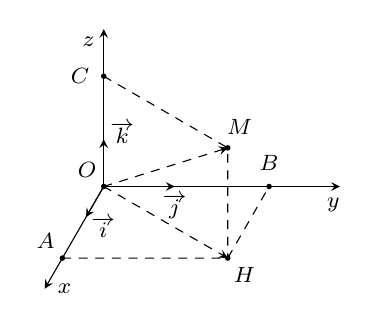
\begin{tikzpicture}[scale=1,>=stealth, font=\footnotesize, line join=round, line cap=round,declare function={a=1.5;b=3;c=2;ga=-120;gb=0;gc=90;}]
			\path
			(0,0) coordinate (O);
			\foreach \g/\d/\t/\p/\v in{-120/1.5/x/A/i,0/3/y/B/j,90/2/z/C/k}
				{\path (O)+(\g:\d) coordinate (\t)
					(O)+(\g:0.7*\d) coordinate (\p)
					(O)+(\g:0.3*\d) coordinate (\v);}
			\path
			(barycentric cs:A=1,O=-1,B=1)coordinate(H)
			(barycentric cs:A=1,B=1,C=1,O=-2)coordinate(M)
			;
			\draw[dashed] (A)--(H)--(B) (C)--(M)--(H);
			\foreach \p/\g in{x/0,y/-110,z/220}
			\draw[-stealth] (O)--(\p)node[shift={(\g:.25)}]{$\p$};
			\foreach \p/\g in{i/-30,j/-90,k/20}
			\draw[-stealth](O)--(\p)node[shift={(\g:.25)}]{$\overrightarrow{\p}$};
			\draw[-stealth,dashed] (O)--(H);
			\draw[-stealth,dashed] (O)--(M);
			\foreach \p/\g in{O/135,A/135,B/90,C/180,H/-45,M/60}
			\fill(\p)circle(1pt)node[shift={(\g:.3)},scale=1]{$\p$};
		\end{tikzpicture}
	}
	\loigiai{
	Ta có
	\allowdisplaybreaks
	\begin{eqnarray*}
		&&OH=OM\cdot \cos\left(\overrightarrow{OH},\overrightarrow{OM}\right)=50\cdot \cos 48^\circ =50\cdot \cos 48^\circ \approx 33{,}46;\\
		&&OC=MH=OM\cdot \sin\left(\overrightarrow{OH},\overrightarrow{OM}\right)=50\cdot \sin 48^\circ \approx 37{,}16;\\
		&&OA=OH\cdot \cos\left(\overrightarrow{i},\overrightarrow{OH}\right)=33{,}46\cdot \cos 64^\circ =33{,}46\cdot \cos 64^\circ \approx 14{,}67;\\
		&&OB=OH\cdot \cos\left(90^\circ -\left(\overrightarrow{i},\overrightarrow{OH}\right)\right)=33{,}46\cdot \cos(90^\circ -64^\circ)=33{,}46\cdot \cos 26^\circ \approx 30{,}07.
	\end{eqnarray*}
	Suy ra $M(14{,}67;30{,}07;37{,}16)$.\\
	Vậy $S=a+b+c=14{,}67+30{,}07+37{,}16=81{,}9$.
	}
\end{bt}

\begin{bt}%[2D1C5-8]%[KNTT - Lớp 12 - Ôn tập giữa học kì 1 - Đề 2]%[Nguyễn Tấn Linh]
	Một máng nước mưa được làm từ một tấm tôn rộng 45 cm bằng cách gấp hai phía của tấm tôn với kích thước bằng $\dfrac{1}{3}$ tấm tôn sao cho nó tạo thành một góc $x$.
	\begin{center}\begin{tikzpicture}[line join = round, line cap = round,>=stealth,font=\footnotesize,scale=1]
			\def \a{3}
			\def \goc{60}
			\draw (0,0)--++(\a,0) node[midway,below]{$15$ cm} coordinate(A)--++(\a,0) node[midway,below]{$15$ cm} coordinate(B)--++(\a,0) node[midway,below]{$15$ cm};
			\def \r{2}
			\draw (B)--++(\goc:\r) (A)--++({180-\goc}:\r);
			\node at ($(B)+({\goc/2}:0.3)$)[]{$x$};
			\node at ($(A)+({180-\goc+(\goc)/2}:0.3)$)[]{$x$};
		\end{tikzpicture}\end{center}
	Hỏi phải chọn $x$ bằng bao nhiêu độ để máng chứa được lượng nước mưa tối đa.
	% \shortans{$60$}
	\loigiai{
		\begin{center}\begin{tikzpicture}[line join = round, line cap = round,>=stealth,font=\footnotesize,scale=1]
				\def \a{3}
				\def \goc{60}
				\draw (0,0)--++(\a,0) node[midway,below]{$15$ cm} coordinate(A)--++(\a,0) node[midway,below]{$15$ cm} coordinate(B)--++(\a,0) node[midway,below]{$15$ cm};
				\def \r{2}
				\draw (B)--++(\goc:\r) coordinate(C) (A)--++({180-\goc}:\r) coordinate(D);
				\coordinate (H) at ($(D)!(A)!(C)$);
				\draw (D)--(C) (A)--(H);
				\node at ($(B)+({\goc/2}:0.3)$)[]{$x$};
				\node at ($(A)+({180-\goc+(\goc)/2}:0.3)$)[]{$x$};
				\foreach \diem/\goc in {A/45,B/135,D/90,H/90,C/90} \fill[black](\diem) circle (1pt) ($(\diem)+(\goc:3mm)$) node{$\diem$};
			\end{tikzpicture}\end{center}
		Mặt cắt ngang của máng nước mưa là hình thang cân $ABCD$ như hình vẽ.\\
		Dễ thấy $x\in \left[0^\circ;180^\circ\right]$.\\
		Để máng nước chứa được lượng nước mưa tối đa thì diện tích $ABCD$ là lớn nhất.\\
		Kẻ $AH\perp CD,H\in CD$.\\
		Vì $AB\parallel CD$ nên $\widehat{D}=x$.\\
		Suy ra $AH=AD.\sin D=15.\sin x$, $DH=AD.\cos D=15.\cos x$.\\
		Ta có $CD=AD+2\cdot DH=15+2\cdot 15\cdot \cos x=15+30\cdot \cos x$.\\
		$S_{ABCD}=\dfrac{1}{2}\cdot \left(AB+CD\right)\cdot AH=\dfrac{1}{2}\cdot \left(15+15+30\cdot \cos x\right)\cdot 15\sin x=225\left(\sin x+\dfrac{1}{2}\sin 2x\right)$.\\
		Đặt $f(x)=225\left(\sin x+\dfrac{1}{2}\sin 2x\right)$.\\
		Ta có $f'\left(x\right)=225\left(\cos x+\cos 2x\right)$.\\
		\begin{align*}
			f'\left(x\right)=0 & \Leftrightarrow \cos x+\cos 2x=0                  \\
			                   & \Leftrightarrow 2\cos^2x+\cos x-1=0               \\
			                   & \Leftrightarrow \hoac{              & \cos x=-1   \\&\cos x=\dfrac{1}{2}} \\
			                   & \Rightarrow \hoac{                  & x=180^\circ \\&x=60^\circ.}
		\end{align*}
		Vì $f\left(0^\circ\right)=0$, $f\left(60^\circ\right)=\dfrac{675\sqrt{3}}{4}$, $f\left(180^\circ\right)=0$ nên diện tích $ABCD$ lớn nhất là $\dfrac{675\sqrt{3}}{4}$ khi $x=60^\circ $.}
\end{bt}
% \label{De4}
% %
% \cleardoublepage
% \setcounter{page}{1}
% \rfoot{Trang \thepage/\pageref{DA4} - Đáp án trắc nghiệm Đề 4}
% \begin{center}
% 	\bfseries ĐÁP ÁN TRẮC NGHIỆM ĐỀ 4
% \end{center}

% \inputansbox{10}{ans/ansDe4-TN4}
% \label{DA4}
% %
